\section{Additional Figures from the Empirical-Literature Context} \label{anexo:currie}

This annex reproduces figures from \textcite{currie2020} used only to contextualize the empirical turn in economics and the diffusion of quasi-experimental methods. They are placed in the annex to keep the main literature review focused on the identification problem addressed in this paper.

\begin{figure}[htbp]
    \centering
    \caption{Applied microeconomics articles in top-five journals}
    \label{fig:currie1}
    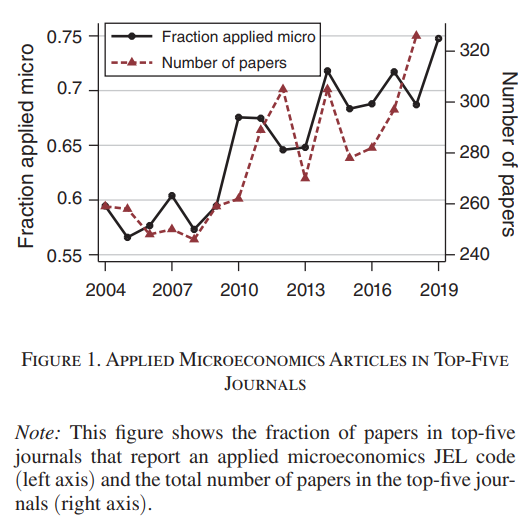
\includegraphics[width=0.7\textwidth]{files/images/figura1currie.png}
    \\ \vspace{0.1cm}
    \footnotesize{\textbf{Source:} \textcite{currie2020}.}
\end{figure}

\begin{figure}[htbp]
    \centering
    \caption{Evolution in the use of quasi-experimental methods}
    \label{fig:currie4}
    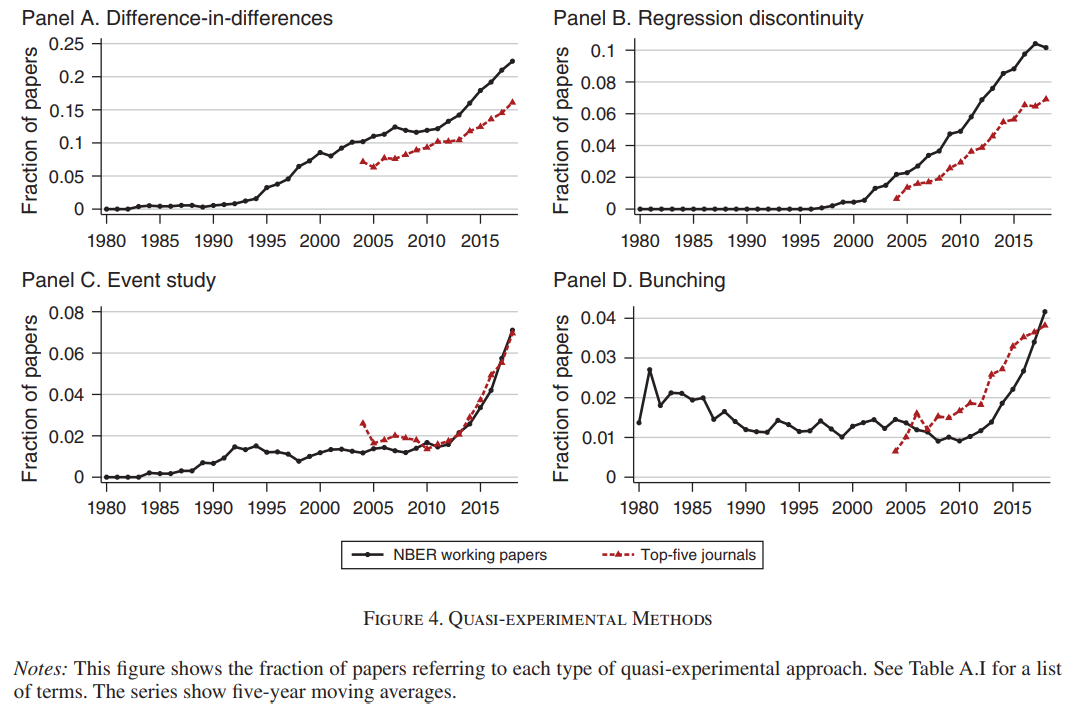
\includegraphics[width=0.9\textwidth]{files/images/figura4currie.png}
    \\ \vspace{0.1cm}
    \footnotesize{\textbf{Source:} \textcite{currie2020}.}
\end{figure}

\begin{figure}[htbp]
    \centering
    \caption{Evolution in the use of terms related to estimate precision}
    \label{fig:currie5}
    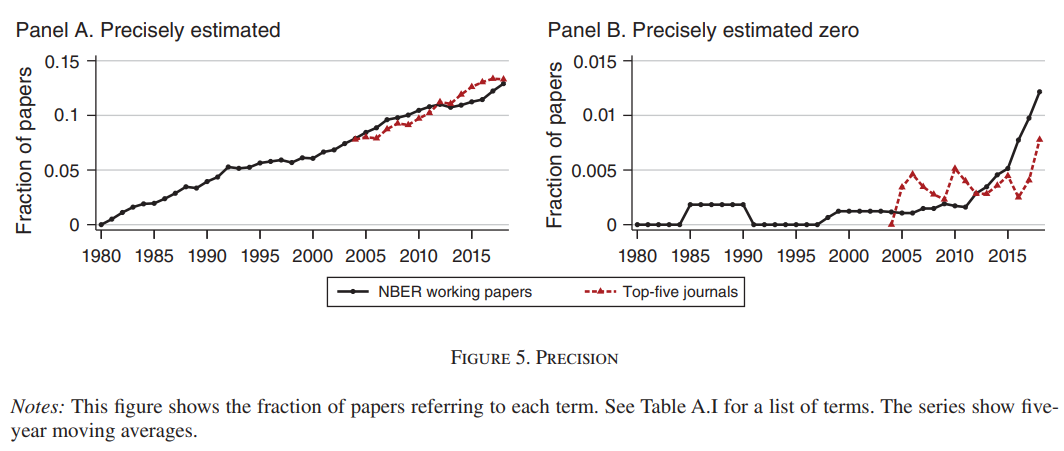
\includegraphics[width=0.9\textwidth]{files/images/figura5currie.png}
    \\ \vspace{0.1cm}
    \footnotesize{\textbf{Source:} \textcite{currie2020}.}
\end{figure}

